\section{特征线法}
\label{sec:transp-characteristics}

速度随位置变化时，粒子的轨迹不再是直线，上一节的公式也就不能直接使用。但“坐在小船上看”的想法仍然有效：沿粒子的轨迹求$u$的变化率，偏微分方程会变成常微分方程。

设曲线$\bm{x}(t)$满足$\dot{\bm{x}}=\bm{v}(\bm{x},t)$。沿这条曲线对$u(\bm{x}(t),t)$求导，由链式法则，
\begin{equation}
  \frac{\mathrm{d}}{\mathrm{d}t}u\bigl(\bm{x}(t),t\bigr)
  =\bigl(\partial_tu+\bm{v}\cdot\nabla u\bigr)\bigl(\bm{x}(t),t\bigr).
  \label{eq:transp-along}
\end{equation}
右端正是输运方程的左端。算子$\partial_t+\bm{v}\cdot\nabla$表示跟随粒子时的变化率，称为\term{物质导数}（material derivative）。

\begin{definition}[特征线]
\label{def:transp-characteristic}
设$\bm{v}$是给定的速度场。常微分方程
\begin{equation}
  \dot{\bm{x}}(t)=\bm{v}\bigl(\bm{x}(t),t\bigr)
  \label{eq:transp-char}
\end{equation}
的解$\bm{x}(t)$在时空中的图像$\{(\bm{x}(t),t)\}$称为输运方程的\term{特征线}（characteristic curve）。
\end{definition}

几何上，特征线是时空向量场$(\bm{v},1)$的积分曲线。图~\ref{fig:transp-chardir}中，$(\bm{v},1)$是特征线的切向量，物质导数是$u$沿这个时空方向的方向导数。输运方程规定的只是这一个方向上的导数，其他方向的导数方程不管。这就是沿特征线可以逐条求解的原因。

\begin{BookInlineFigure}
  \centering
  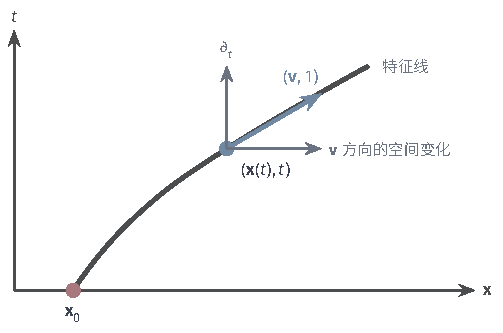
\includegraphics[width=85.2mm]{figures/06-differential-equations/02-partial-differential-equations/tikz/transp-chardir/figure.pdf}
  \caption{时空中的特征线（深灰）。红点是初始位置，蓝色箭头$(\bm{v},1)$是切向量，它由时间方向的一个单位和空间方向的$\bm{v}$合成。物质导数是$u$沿这一方向的方向导数。}
  \label{fig:transp-chardir}
\end{BookInlineFigure}

把偏微分方程沿特征线化为常微分方程，从而逐条求解的方法称为\term{特征线法}（method of characteristics）。

\paragraph{无源输运}
当$f=0$时，式~\eqref{eq:transp-along}说明$u$沿特征线不变。求某点$(\bm{x},t)$的值分三步：解方程~\eqref{eq:transp-char}，得到过这一点的特征线；沿特征线退回到$t=0$，得到出发位置$\bm{x}_0$；令$u(\bm{x},t)=u_0(\bm{x}_0)$。

\begin{example}[均匀拉伸的速度场]
\label{ex:transp-stretch}
取一维速度场$v(x)=x$，初值是以$1$为中心、半宽为$1$的三角形：
\begin{equation}
  u_0(x)=\max\{0,\ 1-\lvert x-1\rvert\}.
  \label{eq:transp-tent}
\end{equation}

特征线满足$\dot{x}=x$，从$x_0$出发的解是
\[
  x(t)=x_0\mathrm{e}^{t}.
\]
反解出发位置，$x_0=x\mathrm{e}^{-t}$。沿特征线$u$不变，于是
\[
  u(x,t)=u_0\bigl(x\mathrm{e}^{-t}\bigr).
\]

在可微的点上代入验证。两个偏导数分别是
\[
  \partial_tu=-x\mathrm{e}^{-t}u_0'\bigl(x\mathrm{e}^{-t}\bigr),\qquad
  x\,\partial_xu=x\mathrm{e}^{-t}u_0'\bigl(x\mathrm{e}^{-t}\bigr),
\]
两者之和为零。

现在算一个具体的点$(x,t)=(3,\ln2)$。特征线的出发位置是$3\mathrm{e}^{-\ln2}=1.5$，所以
\[
  u(3,\ln2)=u_0(1.5)=1-0.5=0.5.
\]
\end{example}

图~\ref{fig:transp-curved}(a)画出了这个例子的特征线。越往右，粒子跑得越快，等间距出发的特征线逐渐散开，解的颜色沿每条特征线不变。(b)是同一个解的剖面：三角形的底从$[0,2]$拉长到$[0,4]$，高度仍然是$1$。(a)中标出的那条特征线把$(1.5,0)$的值$0.5$带到了$(3,\ln2)$，在(b)中对应虚线连接的两点。

\begin{BookInlineFigure}
  \centering
  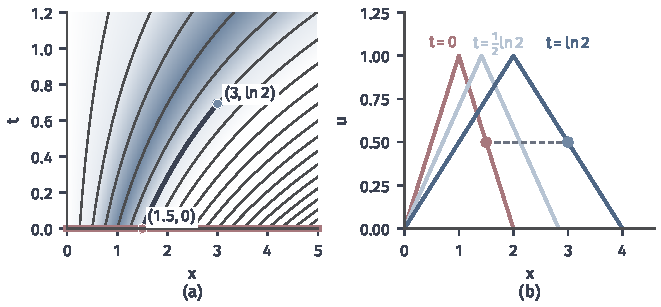
\includegraphics[width=112mm]{figures/06-differential-equations/02-partial-differential-equations/matplotlib/transp-curved/figure.pdf}
  \caption{速度场$v=x$对初值~\eqref{eq:transp-tent}的搬运。(a)特征线$x=x_0\mathrm{e}^{t}$（深灰）和解的时空热图，粗线把$(1.5,0)$（红）连到$(3,\ln2)$（蓝）。(b)初值（红）和$t=\frac12\ln2$、$t=\ln2$的解（蓝色由浅到深），虚线连接同一粒子的前后位置，高度不变。}
  \label{fig:transp-curved}
\end{BookInlineFigure}

速度场显含时间时做法相同，只是特征线的形状要由时间来决定。取$v=\cos t$，特征线$x=x_0+\sin t$来回摆动，解为$u_0(x-\sin t)$。取$v=xt$，特征线是$x=x_0\mathrm{e}^{t^{2}/2}$，解为$u_0(x\mathrm{e}^{-t^{2}/2})$。

图~\ref{fig:transp-timedep}展示了这两种情形。(a)中，每个时刻的速度在空间上处处相同，整个分布作为刚体来回移动。(b)中拉伸的速率随时间增大，特征线弯得越来越厉害。

\begin{BookInlineFigure}
  \centering
  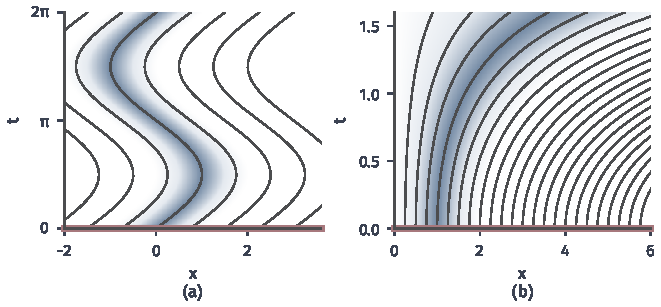
\includegraphics[width=112mm]{figures/06-differential-equations/02-partial-differential-equations/matplotlib/transp-timedep/figure.pdf}
  \caption{显含时间的速度场。深灰线是特征线，蓝色越深值越大，红线是初始线。(a)$v=\cos t$，初值是以$0$为中心、半宽为$1$的三角形。(b)$v=xt$，初值是式~\eqref{eq:transp-tent}。}
  \label{fig:transp-timedep}
\end{BookInlineFigure}

\paragraph{带源项的输运}
有源项时，由式~\eqref{eq:transp-along}，沿特征线的方程变成
\[
  \frac{\mathrm{d}}{\mathrm{d}t}u\bigl(\bm{x}(t),t\bigr)=f\bigl(\bm{x}(t),t\bigr).
\]
右端是沿已知曲线的已知函数，积分即得
\begin{equation}
  u\bigl(\bm{x}(t),t\bigr)=u_0(\bm{x}_0)+\int_0^{t}f\bigl(\bm{x}(s),s\bigr)\,\mathrm{d}s.
  \label{eq:transp-source-along}
\end{equation}
这就是图~\ref{fig:transp-trace}(c)的准确含义：$f$沿轨迹累积到$u$上。

\begin{example}[带源项的计算]
\label{ex:transp-source}
仍取$v=x$与初值~\eqref{eq:transp-tent}，源项取$f(x,t)=x$。沿特征线$x(s)=x_0\mathrm{e}^{s}$，由式~\eqref{eq:transp-source-along}，
\[
  u\bigl(x_0\mathrm{e}^{t},t\bigr)=u_0(x_0)+\int_0^{t}x_0\mathrm{e}^{s}\,\mathrm{d}s=u_0(x_0)+x_0\bigl(\mathrm{e}^{t}-1\bigr).
\]

把$x_0=x\mathrm{e}^{-t}$代回，得到
\[
  u(x,t)=u_0\bigl(x\mathrm{e}^{-t}\bigr)+x\bigl(1-\mathrm{e}^{-t}\bigr).
\]

计算点$(2,\ln2)$。它的出发位置是$x_0=1$，所以
\[
  u(2,\ln2)=u_0(1)+2\cdot\tfrac12=2.
\]
不计源项时，这一点的值是$1$，源项沿特征线累积的贡献是$1$。
\end{example}

图~\ref{fig:transp-source}(b)就是这个累积过程：沿出发于$x_0=1$的特征线，$u$从$1$增长到$\mathrm{e}^{t}$，浅蓝色的面积对应$\int_0^{t}\mathrm{e}^{s}\,\mathrm{d}s$。

\begin{BookInlineFigure}
  \centering
  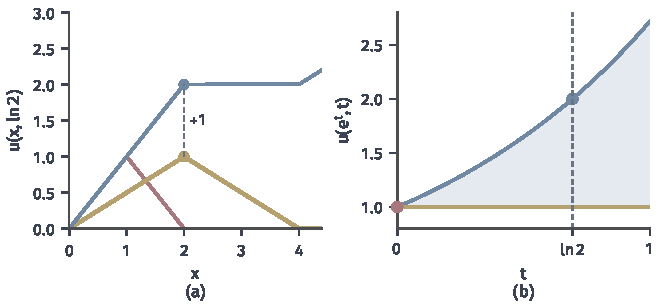
\includegraphics[width=112mm]{figures/06-differential-equations/02-partial-differential-equations/matplotlib/transp-source/figure.pdf}
  \caption{$v=x$、$f=x$的输运。(a)初值（红）、无源解（黄）和有源解（蓝）在$t=\ln2$的剖面，点$x=2$处两解相差$1$。(b)沿特征线$x=\mathrm{e}^{t}$的场值（蓝）与无源时的常值（黄），浅蓝区域是源项的累积，红点是初值。}
  \label{fig:transp-source}
\end{BookInlineFigure}

场的值也可以影响沿途的变化，典型的例子是线性衰减$f=-c(\bm{x},t)\,u+\tilde{f}$。此时沿特征线仍是一个常微分方程，只是变成了线性方程，用积分因子解出：
\begin{equation}
  u\bigl(\bm{x}(t),t\bigr)=\mathrm{e}^{-\int_0^{t}c\,\mathrm{d}r}\,u_0(\bm{x}_0)
  +\int_0^{t}\mathrm{e}^{-\int_s^{t}c\,\mathrm{d}r}\,\tilde{f}\bigl(\bm{x}(s),s\bigr)\,\mathrm{d}s,
  \label{eq:transp-reaction}
\end{equation}
其中$c$沿同一条特征线取值。例如$v=x$，$c=1$，$\tilde{f}=0$时，解为$u=\mathrm{e}^{-t}u_0(x\mathrm{e}^{-t})$。

\paragraph{与经典解的关系}
上面的计算默认了解存在且足够光滑，然后沿特征线推出它的值。这个过程反过来是否成立？按特征线公式造出的函数，是否真的满足方程？这需要速度场和数据的正则性。本章其余部分经常用到下面的条件，这里集中写出。

\medskip
\noindent\textbf{条件（V）.} $\bm{v}:\mathbb{R}^{d}\times[0,T]\to\mathbb{R}^{d}$连续，关于$\bm{x}$连续可微，Jacobian矩阵$\nabla\bm{v}$连续，且存在$L$，使对所有$(\bm{x},t)$有$\lVert\nabla\bm{v}(\bm{x},t)\rVert_2\leq L$。
\medskip

条件（V）说明$\bm{v}$关于$\bm{x}$全局Lipschitz，由第~\ref{chap:ode-existence-continuation}章的整体存在唯一性结论，方程~\eqref{eq:transp-char}过每一点$(\bm{x},t)$恰有一条定义在$[0,T]$上的解，记它在时刻$s$的位置为$\bm{X}(s;\bm{x},t)$。这条解由$\bm{X}(t;\bm{x},t)=\bm{x}$确定。

\begin{theorem}[特征线解与经典解]
\label{thm:transp-classical}
设$\bm{v}$满足条件（V），$u_0\in C^{1}(\mathbb{R}^{d})$，$f$在$\mathbb{R}^{d}\times[0,T]$上连续，关于$\bm{x}$连续可微且$\nabla f$连续。则输运问题~\eqref{eq:transp-ibvp}（$\Omega=\mathbb{R}^{d}$）有唯一的$C^{1}$解，
\begin{equation}
  u(\bm{x},t)=u_0\bigl(\bm{X}(0;\bm{x},t)\bigr)+\int_0^{t}f\bigl(\bm{X}(s;\bm{x},t),s\bigr)\,\mathrm{d}s.
  \label{eq:transp-char-solution}
\end{equation}
\end{theorem}

\begin{proof}
先证唯一性。设$u$是$C^{1}$解。沿过$(\bm{x},t)$的特征线，由式~\eqref{eq:transp-along}和方程，$u$的变化率等于$f$。从$0$到$t$积分，就得到式~\eqref{eq:transp-char-solution}，所以解只能是这个函数。

再证存在性，分两步：先说明这个函数是$C^{1}$的，再验证方程。令
\[
  \bm{\Psi}(\bm{x}_0,t)=\bigl(\bm{X}(t;\bm{x}_0,0),\,t\bigr).
\]
由解对初值的可微性（第~\ref{chap:ode-sensitivity}章），并结合$\partial_t\bm{X}=\bm{v}$，$\bm{\Psi}$是$C^{1}$映射。它的Jacobian矩阵是分块上三角的，对角块分别是$\mathrm{D}_{\bm{x}_0}\bm{X}$和$1$，行列式等于$\det\mathrm{D}_{\bm{x}_0}\bm{X}$，由第~\ref{chap:ode-sensitivity}章的Liouville公式知它恒正。

轨迹唯一性说明$\bm{\Psi}$是$\mathbb{R}^{d}\times[0,T]$到自身的双射。由反函数定理，$\bm{\Psi}^{-1}$也是$C^{1}$的，在$t=0,T$处按单侧导数理解。定义
\[
  W(\bm{x}_0,t)=u_0(\bm{x}_0)+\int_0^{t}f\bigl(\bm{X}(s;\bm{x}_0,0),s\bigr)\,\mathrm{d}s.
\]

$f$关于$\bm{x}$连续可微，所以$W$关于$\bm{x}_0$可以在积分号下求导，并且偏导数连续。$W$关于$t$的偏导数等于被积函数在$s=t$的值，也连续。所以$W\in C^{1}$，从而$u=W\circ\bm{\Psi}^{-1}\in C^{1}$。由于$\bm{X}(s;\bm{x}_0,0)=\bm{X}(s;\bm{x},t)$（同一条特征线），$u$就是式~\eqref{eq:transp-char-solution}的函数。

最后验证方程。由定义，$u(\bm{X}(t;\bm{x}_0,0),t)=W(\bm{x}_0,t)$。对$t$求导，并用式~\eqref{eq:transp-along}，
\[
  \bigl(\partial_tu+\bm{v}\cdot\nabla u\bigr)\bigl(\bm{X}(t;\bm{x}_0,0),t\bigr)=f\bigl(\bm{X}(t;\bm{x}_0,0),t\bigr).
\]
$\bm{\Psi}$是满射，所以方程在每一点成立。$t=0$时，$\bm{X}(0;\bm{x},0)=\bm{x}$，积分为零，初值条件成立。
\end{proof}

条件的作用可以逐一核对。$\bm{v}$的Lipschitz性保证过每点恰有一条特征线，否则“退回到$t=0$”的位置不确定，第~\ref{sec:transp-flow}节会给出具体的反例。$\nabla\bm{v}$的连续性让特征线关于初值$C^{1}$，这是解可微的来源。

$u_0$的$C^{1}$要求不能去掉。例~\ref{ex:transp-stretch}的三角形初值在$x=0,1,2$有折角，公式给出的解沿相应的三条特征线也有折角，它只在这些线之外是经典解。这说明特征线公式可以比方程本身走得更远，第~\ref{sec:transp-weak}节用测试函数解释这种解。有界区域的情形要把积分的下限换成特征线离开区域的时刻，并要求初值和入流数据在角点上按第~\ref{sec:transp-problem}节的方式衔接。
